\documentclass{standalone}
\usepackage{graphicx}	
\usepackage{amssymb, amsmath}
\usepackage{color}
\usepackage{wasysym}

\usepackage{tikz}
\usetikzlibrary{intersections, backgrounds}
\usepackage{pgfmath}

\definecolor{light}{RGB}{220, 188, 188}
\definecolor{mid}{RGB}{185, 124, 124}
\definecolor{dark}{RGB}{143, 39, 39}
\definecolor{highlight}{RGB}{180, 31, 180}
\definecolor{gray10}{gray}{0.1}
\definecolor{gray20}{gray}{0.2}
\definecolor{gray30}{gray}{0.3}
\definecolor{gray40}{gray}{0.4}
\definecolor{gray60}{gray}{0.6}
\definecolor{gray70}{gray}{0.7}
\definecolor{gray80}{gray}{0.8}
\definecolor{gray90}{gray}{0.9}
\definecolor{gray95}{gray}{0.95}

\newcommand*{\offset}{0.025}

\begin{document}

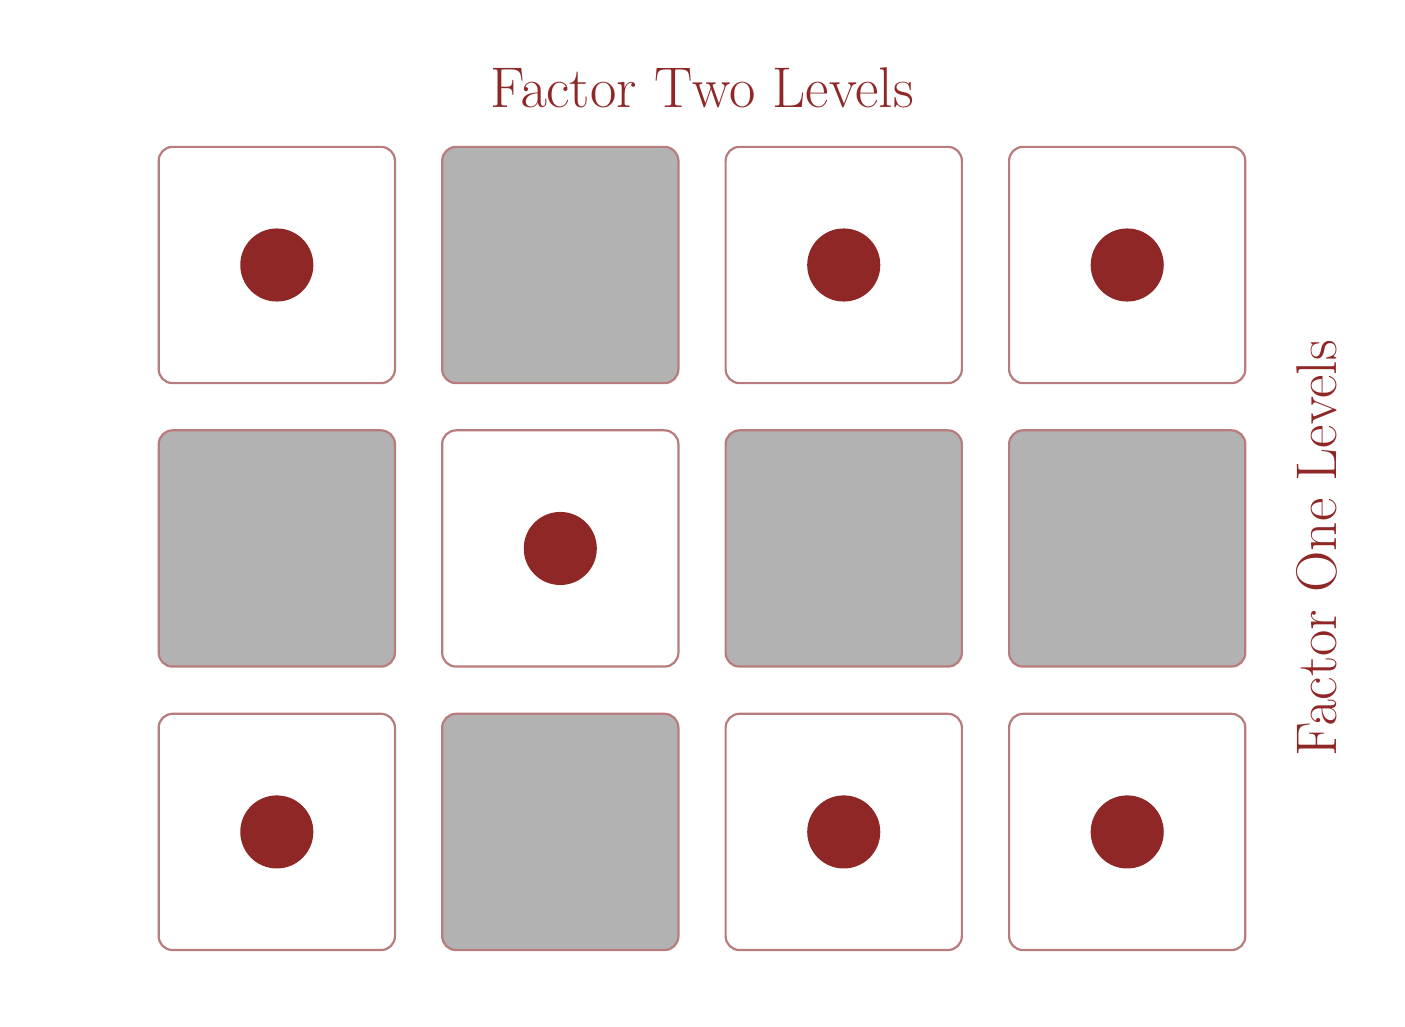
\begin{tikzpicture}[scale=0.3, thick]

\pgfmathsetmacro{\cx}{2}
\pgfmathsetmacro{\cy}{3}

\draw[white] (-28.5, -19) rectangle (28.5, 22);

\node[dark, rotate=90] at (26, 0) { \huge Factor One Levels };
\node[dark] at (0, 19.5) { \huge Factor Two Levels };

\pgfmathsetmacro{\x}{-6}
\pgfmathsetmacro{\y}{12}
\fill[gray70, rounded corners=5] (-5 + \x, -5 + \y) rectangle +(10, 10);

\pgfmathsetmacro{\x}{-18}
\pgfmathsetmacro{\y}{0}
\fill[gray70, rounded corners=5] (-5 + \x, -5 + \y) rectangle +(10, 10);

\pgfmathsetmacro{\x}{6}
\pgfmathsetmacro{\y}{0}
\fill[gray70, rounded corners=5] (-5 + \x, -5 + \y) rectangle +(10, 10);

\pgfmathsetmacro{\x}{18}
\pgfmathsetmacro{\y}{0}
\fill[gray70, rounded corners=5] (-5 + \x, -5 + \y) rectangle +(10, 10);

\pgfmathsetmacro{\x}{-6}
\pgfmathsetmacro{\y}{-12}
\fill[gray70, rounded corners=5] (-5 + \x, -5 + \y) rectangle +(10, 10);

\foreach \x in {-18, -6, 6, 18} {
  \foreach \y in {-12, 0, 12} {
    \draw[mid, rounded corners=5] (-5 + \x, -5 + \y) rectangle +(10, 10);
  }
}

\filldraw[draw=dark, fill=dark] (-18, 12) circle (1.5);
\filldraw[draw=dark, fill=dark] (6, 12) circle (1.5);
\filldraw[draw=dark, fill=dark] (18, 12) circle (1.5);

\filldraw[draw=dark, fill=dark] (-6, 0) circle (1.5);

\filldraw[draw=dark, fill=dark] (-18, -12) circle (1.5);
\filldraw[draw=dark, fill=dark] (6, -12) circle (1.5);
\filldraw[draw=dark, fill=dark] (18, -12) circle (1.5);

\end{tikzpicture}

\end{document}  